\documentclass[11pt,]{article}
\usepackage{lmodern}
\usepackage{amssymb,amsmath}
\usepackage{ifxetex,ifluatex}
\usepackage{fixltx2e} % provides \textsubscript
\ifnum 0\ifxetex 1\fi\ifluatex 1\fi=0 % if pdftex
  \usepackage[T1]{fontenc}
  \usepackage[utf8]{inputenc}
\else % if luatex or xelatex
  \ifxetex
    \usepackage{mathspec}
  \else
    \usepackage{fontspec}
  \fi
  \defaultfontfeatures{Ligatures=TeX,Scale=MatchLowercase}
\fi
% use upquote if available, for straight quotes in verbatim environments
\IfFileExists{upquote.sty}{\usepackage{upquote}}{}
% use microtype if available
\IfFileExists{microtype.sty}{%
\usepackage{microtype}
\UseMicrotypeSet[protrusion]{basicmath} % disable protrusion for tt fonts
}{}
\usepackage[margin=1in]{geometry}
\usepackage{hyperref}
\hypersetup{unicode=true,
            pdftitle={A User-Friendly U.S. Census Browser for R},
            pdfauthor={Kiegan Rice},
            pdfborder={0 0 0},
            breaklinks=true}
\urlstyle{same}  % don't use monospace font for urls
\usepackage{graphicx,grffile}
\makeatletter
\def\maxwidth{\ifdim\Gin@nat@width>\linewidth\linewidth\else\Gin@nat@width\fi}
\def\maxheight{\ifdim\Gin@nat@height>\textheight\textheight\else\Gin@nat@height\fi}
\makeatother
% Scale images if necessary, so that they will not overflow the page
% margins by default, and it is still possible to overwrite the defaults
% using explicit options in \includegraphics[width, height, ...]{}
\setkeys{Gin}{width=\maxwidth,height=\maxheight,keepaspectratio}
\IfFileExists{parskip.sty}{%
\usepackage{parskip}
}{% else
\setlength{\parindent}{0pt}
\setlength{\parskip}{6pt plus 2pt minus 1pt}
}
\setlength{\emergencystretch}{3em}  % prevent overfull lines
\providecommand{\tightlist}{%
  \setlength{\itemsep}{0pt}\setlength{\parskip}{0pt}}
\setcounter{secnumdepth}{0}
% Redefines (sub)paragraphs to behave more like sections
\ifx\paragraph\undefined\else
\let\oldparagraph\paragraph
\renewcommand{\paragraph}[1]{\oldparagraph{#1}\mbox{}}
\fi
\ifx\subparagraph\undefined\else
\let\oldsubparagraph\subparagraph
\renewcommand{\subparagraph}[1]{\oldsubparagraph{#1}\mbox{}}
\fi

%%% Use protect on footnotes to avoid problems with footnotes in titles
\let\rmarkdownfootnote\footnote%
\def\footnote{\protect\rmarkdownfootnote}

%%% Change title format to be more compact
\usepackage{titling}

% Create subtitle command for use in maketitle
\newcommand{\subtitle}[1]{
  \posttitle{
    \begin{center}\large#1\end{center}
    }
}

\setlength{\droptitle}{-2em}
  \title{A User-Friendly U.S. Census Browser for R}
  \pretitle{\vspace{\droptitle}\centering\huge}
  \posttitle{\par}
  \author{Kiegan Rice}
  \preauthor{\centering\large\emph}
  \postauthor{\par}
  \date{}
  \predate{}\postdate{}

\usepackage{float}

\begin{document}
\maketitle

\subsection{Introduction}\label{introduction}

Census data is an important snapshot of information about a country at
different times throughout their history. It is an integral part of
keeping track of the history of a country and the people who occupy it,
as it gives us records of the occupants of a country and how they live
their lives. The value of census data to a country and its citizens is
difficult to overstate. Many recognize the usefulness of the census
data, especially when aggregated and presented in a way that allows for
viewers to learn something new about the world around them. While the
history books we learn from in high school present us with a narrative
of the events that occured, students often don't get to interact with
the raw data ourselves in that learning environment. Accessible and
usable census data allows the exploration of different demographic
groups over time, or investigations of a particular period of time and
what the demographic and economic landscape looked like in the past.
Even today, for those who can't travel the world, data about the world
around them could allow them to learn more about those places and learn
something more about groups of people they may not usually engage with.

From an early point in the United States' history, there were ``many
eminent men of science'' who recognized the value of the census data and
worked to aggregate and present the data that had been collected on the
population. Francis A. Walker's ``Statistical Atlas of the United
States'', based on the 1870 census, was an impressive effort in
aggregating population data to present it in a visually appealing way.
Although the Census Bureau's ``Statistical Atlases'' eventually stopped
being made, they were an important start to the effort of presenting
census data to a wider public.

Today, as methods of data analysis and visualization continue to be
developed and improved, access to census data allows us to look back on
that history and explore, synthesize, and visualize the information to
learn more about patterns in many different parts of the population.

\emph{Mention Dr.~Hofmann's paper to improve the Statistical Atlas here}

\begin{itemize}
\item
  Ever-changing census means that we have different information in
  different years
\item
  To get complete information, we have to be able to see what
  information we have and don't have
\end{itemize}

An inherent problem in census data is that a country's census changes
over time; the variables collected, how they are collected, and even the
locations they are collected for change as the country is formed, and
subsequently grows and changes. The United States census data is no
exception to this rule. In a little under two and a half centuries, the
census has taken on many different forms. Data on occupations has
transformed as the employment landscape has changed; new states have
been formed, the most recent being within the last 100 years;
definitions of various demographic groups and the terminology used to
describe them have been updated as the demographic makeup of the country
has changed. Each decennial census brings a different set of variables
to the table. Sometimes these variables are new things the Census Bureau
is interested in learning, while sometimes they remove variables that
are no longer relevant or whose information is captured somewhere else.

Unfortunately, because the founders of the U.S. Census were unable see
200 years into the future, those interested in working with census data
are left with quite the inescapable mess. If you want to focus in on a
particular demographic group and their journey as part of the population
of the United States, you may have ten or more different variables names
to describe that one group over the course of the census from 1790 to
1960 - and that is just for one single group! Of course, we cannot just
simply change variable names to match our own research needs. It is
important to keep the data in its true form and be honest to the way
that the population was defined at different times throughout history,
even if our instinct may be to `clean' the data by changing variable
names.

\subsection{Background ?(Literature
Review)?}\label{background-literature-review}

The University of Virginia Library hosted a ``Historical Census
Browser'' for many years that allowed users to search United States
Census Data for use in research, teaching, and personal inquiry. The
data included data on various aspects of the U.S. population from the
1790 Census through the 1960 Census. This Historical Census Browser was
free and available for use for anyone with an internet connection. This
Census Browser allowed a user to peruse available topics for each census
year, at both the state and county levels. The Historical Census Browser
was taken down on December 31, 2016, with the county-level aggregated
data becoming unavailable several months before this. The source was
widely used, with several other university libraries and educational
resources including University of California Santa Barbara, University
of Pennsylvania, University of Michigan(University of Michigan
Population Studies Center 2017), and the Smithsonian's History Explorer
directing researchers to use the University of Virginia source.

\emph{Look into what other things are available, different sources of
data (NHGIS at U of Minn., different license). What issues there are
with different sources of data}

\subsection{Work}\label{work}

\subsubsection{Motivation}\label{motivation}

The University of Virginia Libraries website now directs users to
``Social Explorer'' or the ``National Historical Geographic Information
System'' website. However, neither resource provides the full advantages
that the Historical Census Browser offered: a free-to-use and
user-friendly data browser that allows users to choose which data they
are interested in using, and download the complete records for their own
independent use.

\subsubsection{Description}\label{description}

Although the county-level data had already been removed from the
website, the state-level aggregated records for each decennial census
from 1790 through 1960 were captured from the website in September of
2016 and saved as raw data with the intent to create a resource for R
users that allowed the same main functionalities of the original
University of Virginia Historical Census Browser, streamlined for easy
data searches and data management.

\begin{itemize}
\tightlist
\item
  What the package includes and what capabilities the Shiny app has
\end{itemize}

\subsubsection{Example}\label{example}

In the Shiny app, we can choose to focus in on a single year of the
census or look for data across a range of years. We can easily use the
``Get Your Data'' Shiny app to search for a topic of interest, find the
data we want, download state-level information, and tell a visual story
of populations in the United States over time. To demonstrate the
all-knowing power of this Shiny app, we will walk through an example on
the history of the African American population in the United States. We
begin by running the shiny app:

\begin{verbatim}
put code chunk to run shiny app here
\end{verbatim}

The default set of years is 1790 to 1920. However, we can easily expand
the slider range to be able to explore data across all the available
years, 1790 to 1960. We can also order by how the ``Total'' column, or
how many of years each of the variables appear in. These variables
appear on the left side of the table, as rows.

\begin{figure}[htbp]
\centering
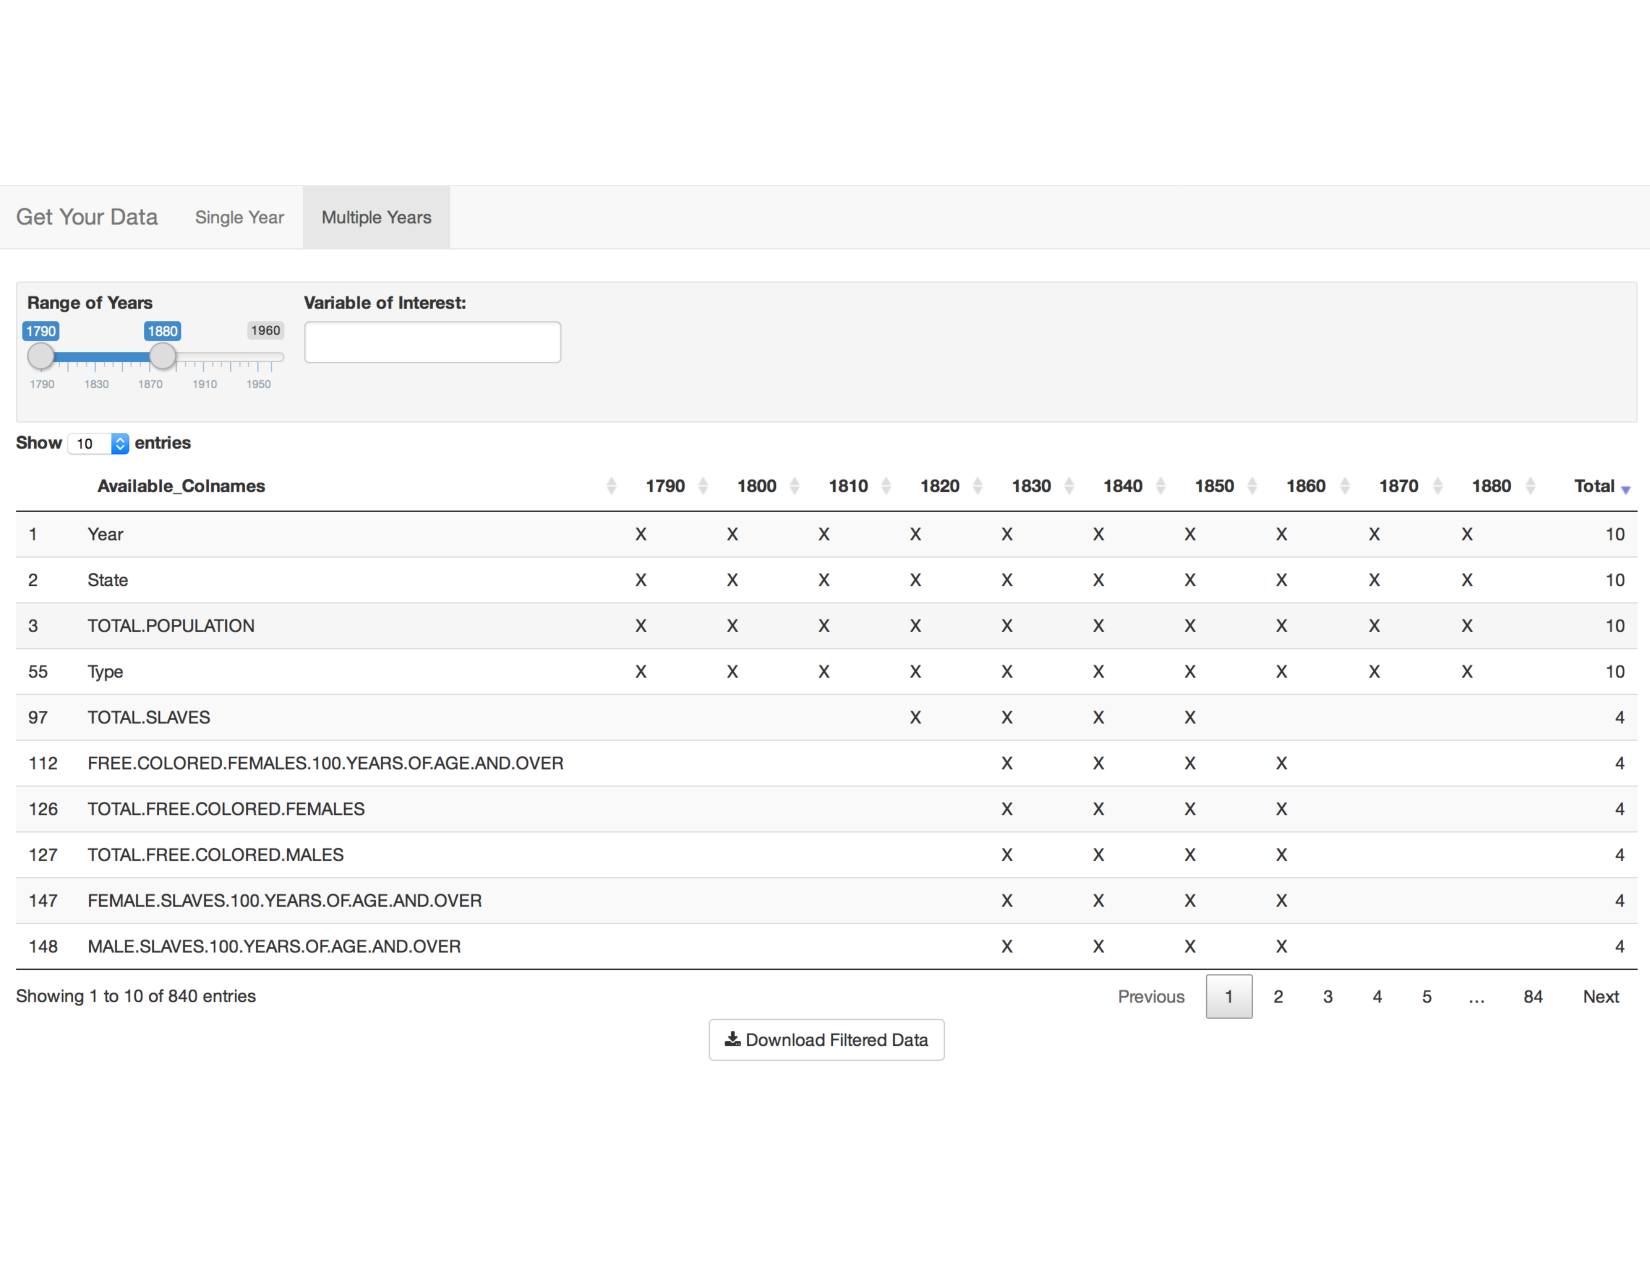
\includegraphics{./figures/app-sshot-1790-to-1880.pdf}
\caption{An example of available column names for the years 1790 to
1880.}
\end{figure}

The available variable names here are already ordered by how many years
they appear in, so we can see right off the bat that we have a serious
lack of variable continuity. The identifying variables that appear each
year ar \texttt{YEAR}, \texttt{STATE}, \texttt{TOTAL.POPULATION}, and
\texttt{TYPE}. That means the total number of times they appear is 10,
the number of census years we are looking at. After that, the next most
common variable only appears in 4 of the 10 years we have chosen. That
means we are up against some pretty significant hurdles to track any
demographic group over time.

For now, we are focusing in on African Americans throughout U.S.
history, which means we need to start with the term \texttt{SLAVE} in
the early years of the U.S. census. The vast majority of African
Americans were slaves when the United States was founded, so variables
that count the number of slaves are important variables to have in order
to get a grasp on the African American population in early U.S. history.

Once we have our range of years chosen, we simply enter a search term.
\textbf{All variable names are in all caps, so search in all caps}.
Searching for \texttt{SLAVE} gives us a list of all the possible
variable names across all years, and we can again sort by how how many
years each variable name appears in. Users are then able to click each
of the variables they are interested in, and select
\texttt{Download\ Data} in order to download a .csv file with the data
for all states in the selected years. This .csv file will also always
include the columns \texttt{YEAR}, \texttt{STATE},
\texttt{TOTAL.POPULATION}, and \texttt{TYPE}, even if they are not
selected by the user.

For this example, I executed three separate searches within the
\texttt{Get\ Your\ Data} app, using three different terms that were used
to refer to African Americans at different points in the decennial
census. This gave me three separate .csv files, which I was able to
easily combine using \texttt{full\_join} from the \texttt{dplyr}
package. Now, for an entire demographic group, all of the
state-aggregated population counts are together in one data frame,
although different terms are used at different points in time.

We can now begin to explore this data. We can very easily plot
state-level counts of the \texttt{SLAVES} variable for the year 1790. We
recommend the use of the \texttt{USAboundaries} package in concert with
this census browser, as it provides the most accurate boundaries of the
United States at any given date, and it is important to realize that
values in the data are for the states \emph{as they were} during that
census, not the current (2017) boundaries of the states.

\begin{figure}[htbp]
\centering
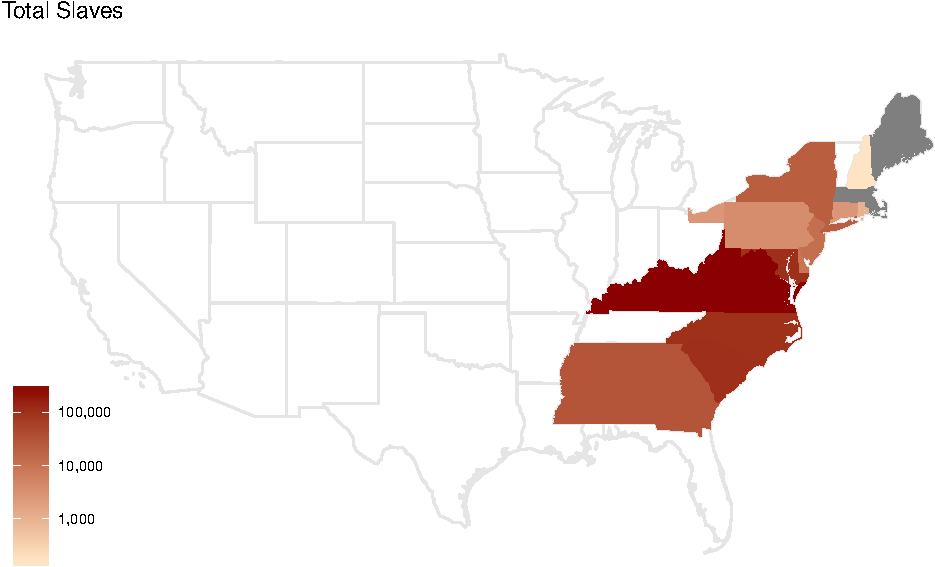
\includegraphics{writeup_files/figure-latex/chunk-1790-map-1.pdf}
\caption{Total number of slaves per state in 1790, plotted on a
continuous log scale. State boundaries for July 4, 1790 were gathered
from \texttt{USAboundaries} package.}
\end{figure}

\subsubsection{Implementation}\label{implementation}

How to use it - this is the most technical part

\subsection{Discussion of Future Work}\label{discussion-of-future-work}

\begin{itemize}
\tightlist
\item
  County-level data would be great\\
\item
  Current data (up to 2010 Census)
\end{itemize}

\subsection*{References}\label{references}
\addcontentsline{toc}{subsection}{References}

\hypertarget{refs}{}
\hypertarget{ref-UMich-HCB}{}
University of Michigan Population Studies Center. 2017. ``Historical
Census Browser (1790 - 1960).'' Accessed March 27.
\url{http://www.psc.isr.umich.edu/dis/data/resource/detail/1369}.


\end{document}
